\documentclass{article}

\usepackage[margin=1in]{geometry}
\usepackage{graphicx} 
\usepackage{gensymb}
\usepackage{amsmath}
\usepackage{multicol}
\usepackage[font=small,labelfont=bf]{caption}
\usepackage{mwe}
\usepackage{graphicx}
\usepackage{tikz}

\title{Introduction}

\begin{document}
\begin{center}
    {\huge{Introduction}}
\end{center}    
    
    Financial time series are beneficial for various purposes, for example to train machine learning models or to be used as inputs in market simulators. In these applications, the constraint of limited availability of large amounts of data can have an impact on the performance of the analysis. For these reasons, models, especially deep-learning ones, tend to overfit and struggle at generalizing. By augmenting a dataset we can contribute to the solution of this issue by providing a larger amount of data with respect to what is already accessible. Thanks to this result, companies can effectively  improve models and also use it to enhance strategy backtesting. 
    \subsection*{Characteristics of Time series}
    GANs can capture the temporal structures of financial time-series so as to generate the major stylized facts of price returns, including the linear unpredictability, the fat-tailed distribution, volatility clustering, the leverage effects, the coarse-fine volatility correlation, and the gain/loss asymmetry. 
    \begin{center}
        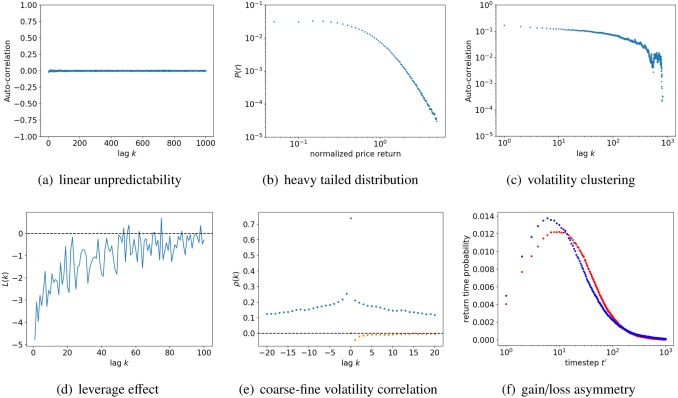
\includegraphics[scale = 0.7]{ts.jpeg}
    \end{center}
    In the studies of financial time-series, there are two major approaches, namely stochastic processes, and agent-based models, for modeling the financial time-series. However, it is difficult to recover all the major stylized facts with such explicit mathematical formulations. As an alternative approach, GANs have shown spectacular ability in the generation of data including realistic image, audio, natural language text, and financial data.\\
   
    \subsection*{General idea for the data}
    We began by taking a dataset of value stocks from the S&P 500 as we assumed it would have been easier to analyze financial series with more convenient intrinsic properties such as moderate volatility. In this way it was easier to interpret the results of our model since we could identify out of range peaks very easily. The reasoning behind was due to the fact that it is very hard to judge the performance of a model like this without a defined metric. As for now, we rely on our visual interpretation.\\ 
    
    \subsection*{Scalar method}
    Since the aim of the project is to augment a dataset to be used for further analysis in machine learning, we want to select the generated data that maintain the statistical properties mentioned above. For this reason we will apply a correction algorithm to correct the range of peaks of volatility. We could better observe the results thanks to the choice of our first dataset of stocks with low volatility. It was possible to capture the strange pattern of the series generated since some results did not mimic correctly  the normal behavior of certain types of stocks.\\ 
    
    \subsection*{Further implementation}
   We are now conducting more trials on different types of financial series starting from very volatile stocks. We would like to understand if the performance of the GAN is altered and then explore solutions on how to fix this, if this is the case.  In the future, our next step is to analyze the results of the series obtained with R, to analyze the statistical properties of the series. We would also like to develop a metric to evaluate accurately the performance of the model.\\

    \subsection*{Implementation and Analysis}
    GANs were first used to give images as output so it can be hard to model different kinds of data. In our case we first tried to input prices to get back a financial series that could still preserve the statistical porperties of what we used as input. Unfortunately this was not the case as the series that did not mimic well the real dataset. In fact we can see how the mean was fixed around zero. Of course, there is a mathematical explanation behind this and we will discuss this topic in subsequent chapters.\\
    
    \begin{center}
        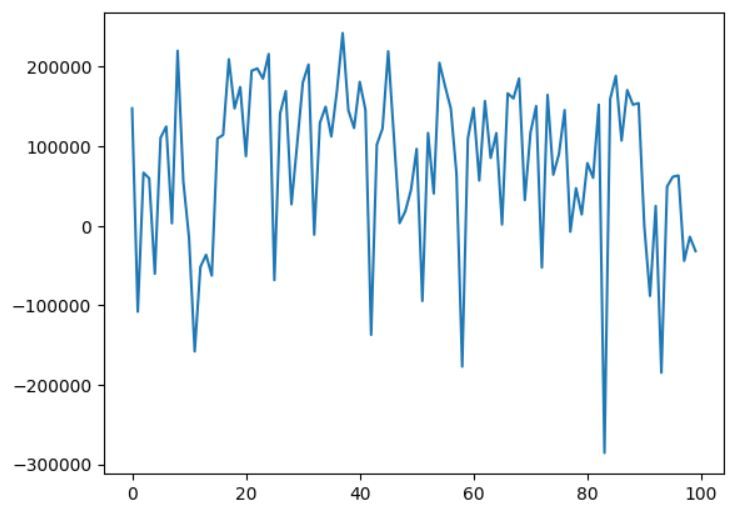
\includegraphics[scale = 0.4]{price.jpeg}
    \end{center}

    Then, we decided to train the model using net returns which worked and therefore we continued our analysis with these data. As we went on with the implementation of the model, we encountered a problem in terms of randomization.\\

    \begin{center}
        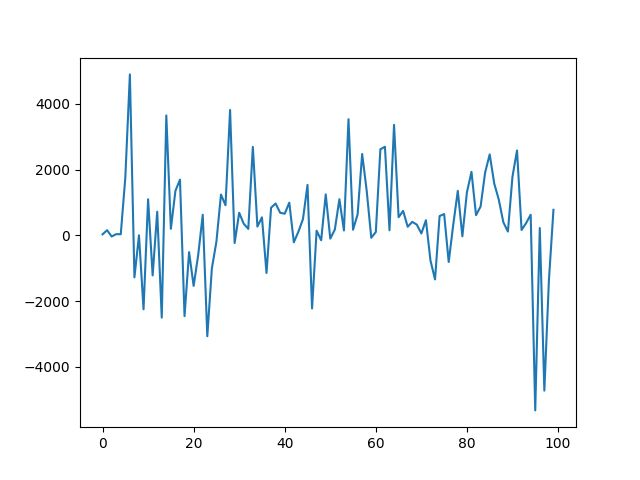
\includegraphics[scale = 0.4]{1.jpg}
        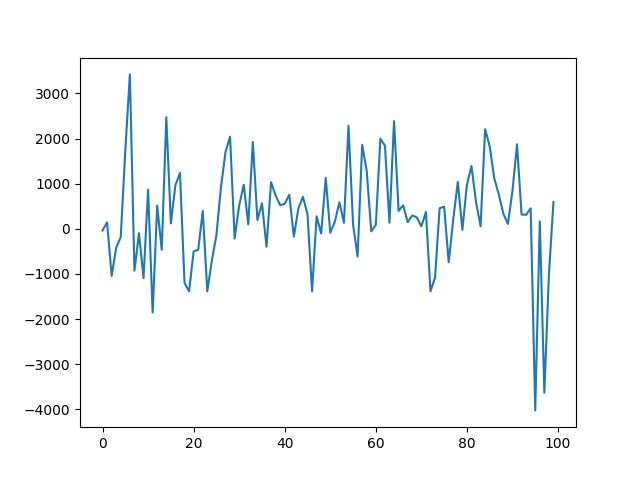
\includegraphics[scale = 0.4]{2.jpg}
        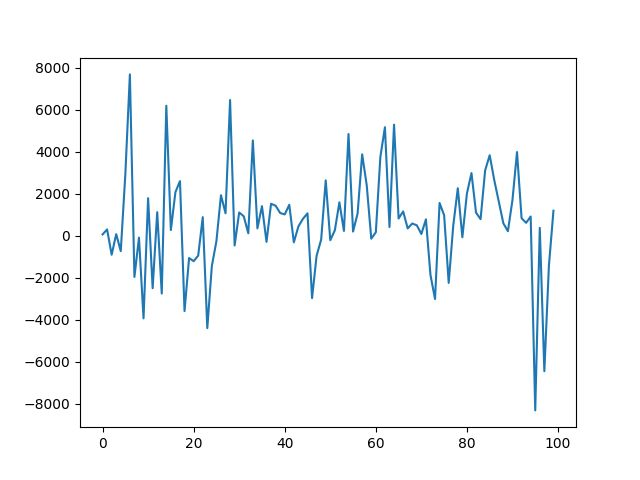
\includegraphics[scale = 0.4]{3.jpg}
        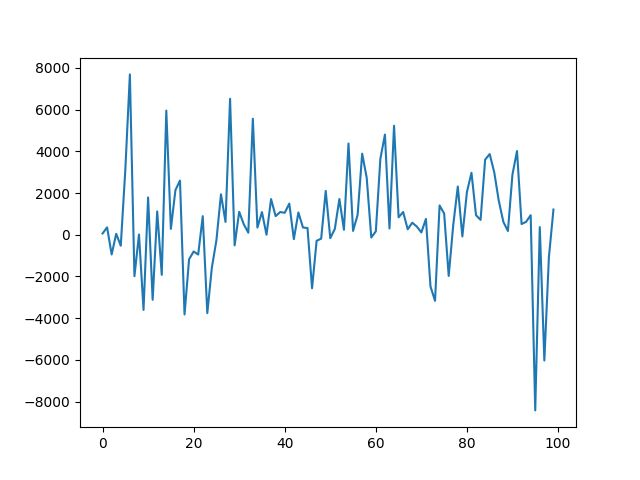
\includegraphics[scale = 0.4]{4.jpg}
    \end{center}\\

    In order to solve this problem we took away the spectral normalization from the generator after doing some trials also with respect to the discriminator. At the end of this process we finally got realistic results which will be shown later in the paper. It is also with these results that we applied the scalar method explained later. \\

    On the other side, we also tried to test the model on log returns with negative results.\\

    \begin{center}
        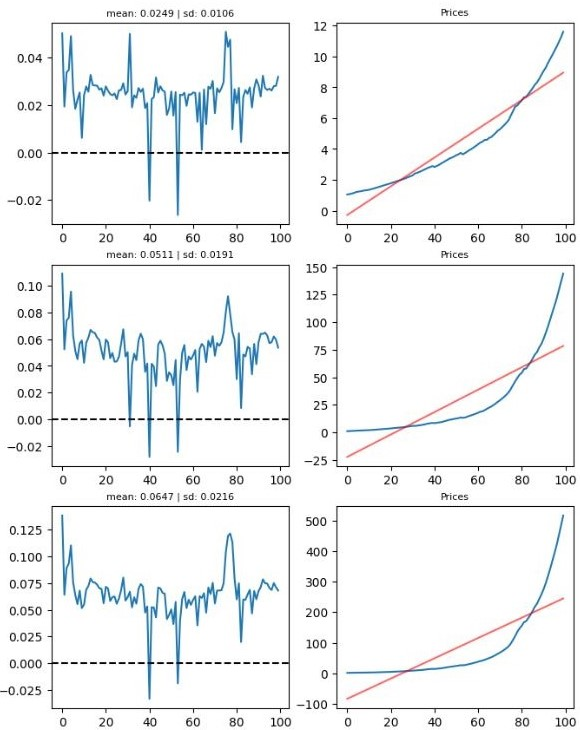
\includegraphics[scale = 0.5]{log.jpeg}
    \end{center}\\

    The mean is not around zero as with the net returns. We will now discuss more about these results by comparing the tyoes of returns to be used in financial data analysis.\\

    \subsection*{Returns}
    Prices between assets may be difficult to compare. For example, a large company might have a higher stock price than a smaller competitor. However, the bigger company’s price could be relatively stable, while the competitor’s smaller price is rapidly increasing. Thus, it is natural to want to think of prices in relative terms. Let's denote the price of an asset at time t. Then the return of an asset captures these relative movements and is defined as:

    \begin{center}
        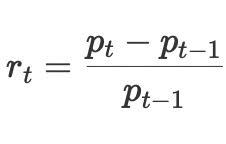
\includegraphics[scale = 0.4]{unnamed.jpg} 
    \end{center}\\
    In words, a return is the change in price of an asset, relative to its previous value. In practice, “returns” often means “log returns”. Log returns are defined as:\\
    \begin{center}
        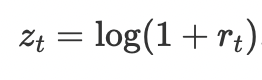
\includegraphics[scale = 0.8]{r.jpg} 
    \end{center}\\
    Returns are lower-bounded by −1.0. One cannot lose more than all of one’s money. However, log returns have an infinite support. And since the log function suppresses big positive values while emphasizing small negative values, log returns are more symmetric than returns. This is a natural consequence of logarithms.\\
    In terms of distribution, net returns follow the normal distribution which is symmetric. The lognormal distribution (of log/geometric returns) is not. It's slightly skewed/biased. It happens because the log function is concave around 1, which means it returns "more negative" numbers for values less than 1 than the positive values it returns for numbers the same distance greater than 1. What that means in a practical sense is that when simple returns average zero, log returns are negative, since negative returns have a more negative log return than "equal" positive returns. If your arithmetic mean is positive but close to zero, then it's not unusual to have a small negative log return average. 
    
    \subsection*{Statistical properties of financial time series}
    The final goal related to the implementation of a GAN is to preserve the statistical properties of the data used. We will list the ones that should be used to evaluate the results. Even though we will limit our evaluation to a qualitative visual interpretation, it is our plan to work on accurate mathematical metrics. We list the three main properties. \\
    \subsection*{linear unpredictability}
    The first fundamental property of financial time-series is its linear unpredictability. This property is quantified by the diminishing auto-correlation function of price return. \\
     \begin{center}
        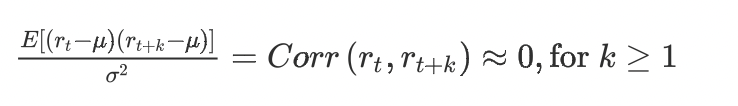
\includegraphics[scale = 0.8]{lp.jpg} 
    \end{center}\\
    The figure shows the decay of the auto-correlation function of the price return in daily scale. The absence of linear correlation in the price return in daily scale implies that the financial markets are efficient to a certain extent.\\
    \subsection*{Fat-tailed distribution}
    The probability distribution has a power-law decay in the tails. A heavy tailed distribution has tails that are heavier than an exponential distribution.  In other words, the tails simply look fatter. As the tails have more bulk, the probability of extreme events is higher compared to the normal. 
    \begin{center}
        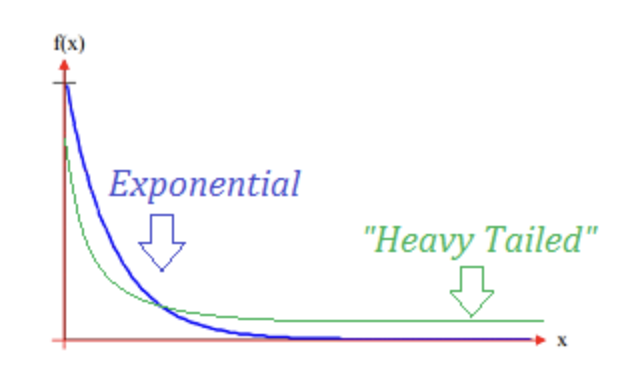
\includegraphics[scale = 0.6]{dist.jpg} 
    \end{center}\\
    

    \subsection*{Volatility clustering}
    While the auto-correlation of the price return is absent, there is still an important temporal structure in the financial time-series, namely volatility clustering. Qualitatively speaking, volatility clustering refers to the fact that the large/small price fluctuations tend to cluster together temporally. Quantitatively, volatility clustering is characterized with the power-law decay of the auto-correlation function of the absolute price returns. 
    \begin{center}
        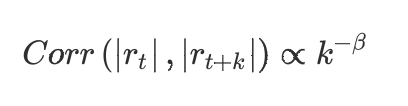
\includegraphics[scale = 0.8]{cl.jpg} 
    \end{center}\\


    
\end{document}
